\documentclass[12pt]{scrartcl}
\usepackage[sexy]{evan}
\usepackage{graphicx}

\usepackage{answers}
\Newassociation{hint}{hintitem}{all-hints}
\renewcommand{\solutionextension}{out}
\renewenvironment{hintitem}[1]{\item[\bfseries #1.]}{}

 %Sets
\newcommand{\N}{\mathbb{N}}
\newcommand{\Z}{\mathbb{Z}}
\newcommand{\F}{\mathbb{F}}
\newcommand{\Q}{\mathbb{Q}}
\newcommand{\R}{\mathbb{R}}
\newcommand{\C}{\mathbb C}
\newcommand{\T}{\mathbb T}
\renewcommand{\hat}{\widehat}
\renewcommand{\tilde}{\widetilde}

\newcommand\at[2]{\left.#1\right|_{#2}}


\let \phi \varphi
\let \mc \mathcal
\let \ol \overline
%From Topology
\newcommand{\cT}{\mathcal{T}}
\newcommand{\cB}{\mathcal{B}}
\newcommand{\cC}{\mathcal{C}}
\newcommand{\cH}{\mathcal{H}}

\newcommand{\supp}{\text{supp }}


\newcommand{\aint}{\mathrel{\int\!\!\!\!\!\!-}}
\let \grad \nabla

\begin{document}
\title{Math 214}
\author{Vishal Raman}
\maketitle
\tableofcontents
\newpage
%\maketitle
\section{Topology}
\begin{definition}[Topological Space] $(X, O_X \subset \mc P(X))$, where $A \in O_x$ are the open sets which satisfy the following:
\begin{enumerate}
\item $\emptyset, X \in O_X$.
\item $A, B \in O_X$ implies $A \cap B \in O_X$
\item $A_i \in O_X$, $i \in I$, then $\bigcup_{i \in I} A_i \in O_X$.
\end{enumerate}
We say that $A \subset X$ is closed if $X \setminus A$ is open.  $U \subset X$ is a neighborhood of $p \in X$ if $\exists A$ such that $p \in A \subset U$.
\end{definition}

\begin{definition}  $\mc B \subset \mc P(X)$ is called a \textbf{basis} for the topology on $X$ if for every subset $A \subset X$, $A$ is open if and only if $A$ is a union of elements of $\mc B$.
\end{definition}

Let $(X, O_X)$, $(Y, O_Y)$ be topological spaces.  

\begin{definition} A function $\phi : X \to Y$ is continuous if for any open subset $B \subset Y$, $\phi^{-1}(B) \subset X$ is open.  
\end{definition}

\begin{definition} $\phi: X \to Y$ is a homeomorphism if it is a continuous bijection whose inverse is continuous.  
\end{definition}

\begin{definition} Let $Y \subset X$ a topological space.  We set $O_Y = \{A \cap Y : A \in O_X\}$.
\end{definition}

\begin{definition} Given a topological space $X$, $X$ is called locally Euclidean (of dimension $n$) at $p \in X$ if there is an open neighborhood about $p \in U \subset X$ that is homeomorphic to an open subset of $\R^n$.
\end{definition}


\begin{definition} A space $X$ is \textbf{Hausdorff} if for any $p, q \in X$, $p \ne q$ there exists open subsets $U, V$ with $p \in U$, $q \in V$ so that $U \cap V = \emptyset$.
\end{definition}

\begin{definition} $K \subset X$ is compact if every open cover of $K$ has a finite subcover.  
\end{definition}

Given a topological space $X$, we have the following definitions:
\begin{definition} $X$ is connected if the only subsets that are open and closed are $\emptyset, X$.
\end{definition}
\begin{definition} A space is path-connected if for any $p, q \in X$ there is a continuous path between them.  
\end{definition}

\begin{definition} An exhaustion by compact subsets is an increasing sequence of subsets $K_1 \subset K_2 \subset \dots \subset X$ such that $K_i$ is compact and $K_i \subset \text{Int}(K_{i+1})$ and $\bigcup_i K_i = X$.
\end{definition}

\begin{definition} Take $\mc U \subset \mc P(X)$.  This is a cover of $X$ if $X = \bigcup_{U \in \mc U} U$.  A collection is called locally finite if every $p \in X$ has a neighborhood $p \in W \subset X$ such that $W$ only intersects finitely many $U \in \mc U$.    
\end{definition}


\begin{definition} A collection of subsets $\mc V$ is called a refinement of some other collection $\mc U$ if for every $V \in \mc V$ there is $U \in \mc U$ such that $V \subset U$.  
\end{definition}
\section{Topological Manifolds}
\begin{definition} A topological space $M$ is called an $n$-dimensional \textbf{topological manifold} if $M$ satisfies the following:
\begin{itemize}
\item $M$ is locally Euclidean at any point,
\item $M$ is Hausdorff,
\item $M$ is second countable.
\end{itemize}
\end{definition}


\begin{definition} A \textbf{coordinate chart} on $M$ is a pair $(U, \phi)$ where $U\subset M$ is open and $\phi: U \to \hat{U} $ is a homeomorphism to an open subset $\hat{U} \subset \R^n$.
\end{definition}

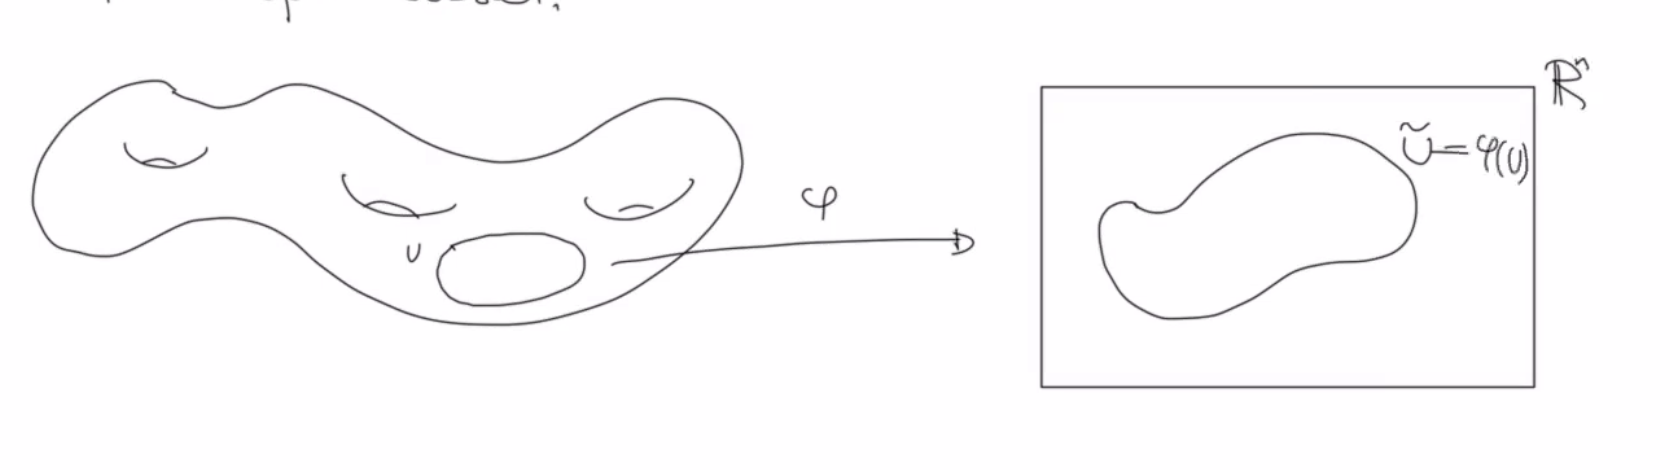
\includegraphics[scale=0.5]{chart.png}

\begin{definition} $X$ is called paracompact if every open cover has a locally finite refinement. 
\end{definition}

\section{Smooth Structures}
\begin{definition} Let $M^n$ be a topological manifold.  Two charts $(U, \phi), (V, \psi)$ of $M$ have a transition map: $\psi \circ \phi^{-1}$.  This map is a homeomorphism.
\end{definition}
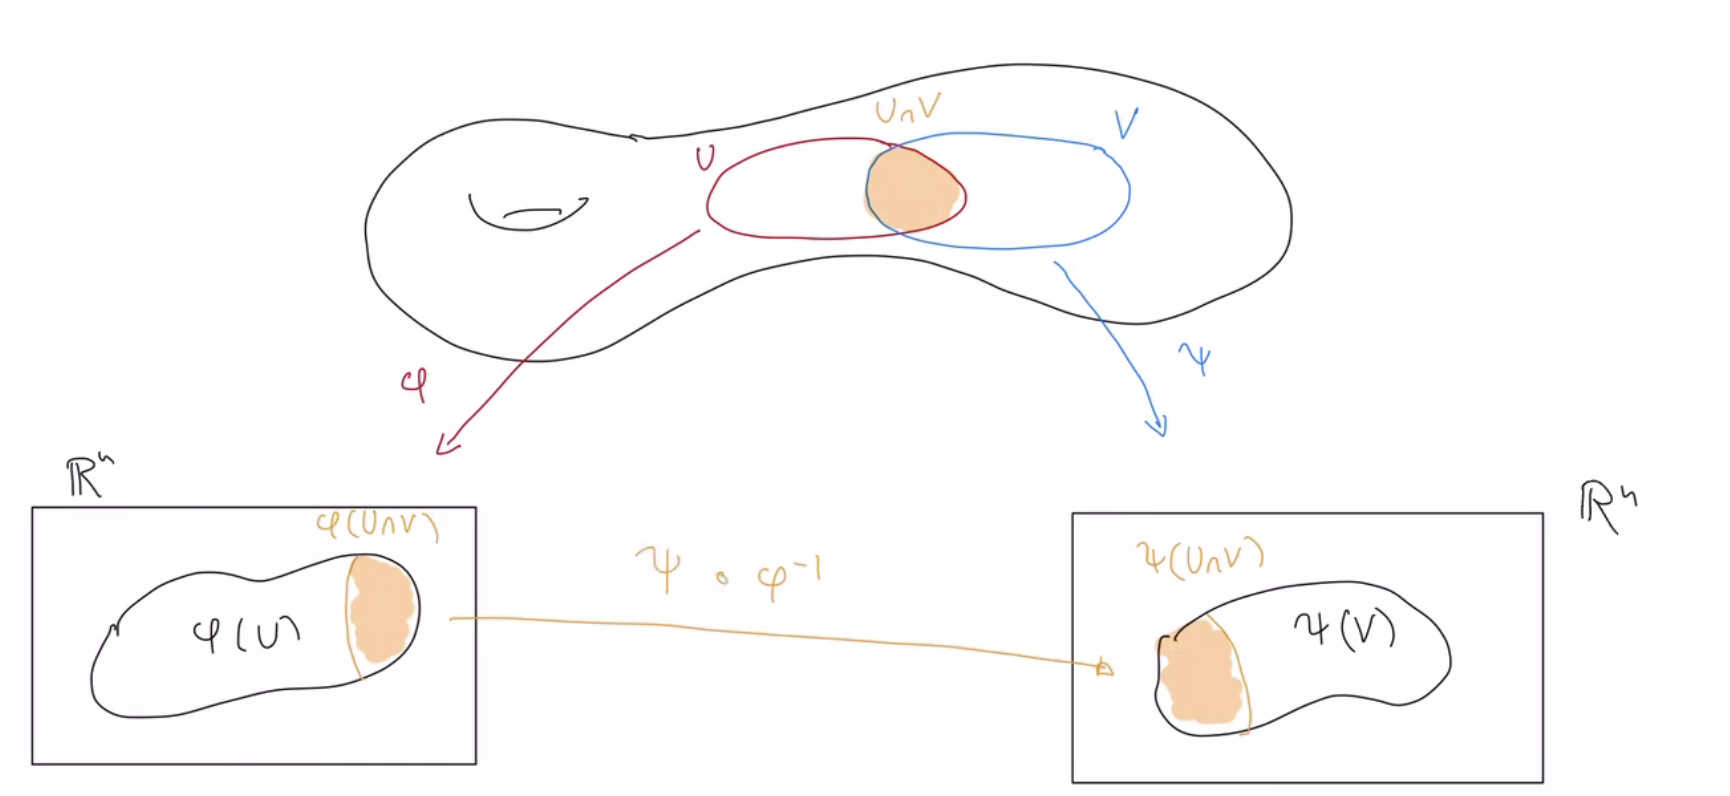
\includegraphics[scale=0.5]{transition}
\begin{definition} Two charts are smoothly compatible if the transition maps in both directions are smooth.
\end{definition}
\begin{definition} An atlas $\mc A$ of $M$ is a collection of charts such that the domains of the charts cover $M$.  An atlas $\mc A$ is smooth if any two charts in $\mc A$ are smoothly compatible.  An atlas $\mc A$ is called a maximal smooth atlas on $M$ if there is no smooth atlas containing $\mc A'$ that contains $\mc A$.  
\end{definition}
\begin{definition} A maximal smooth atlas $\mc A$ on a topological manifold $M$ is called a smooth structure on $M$.
\end{definition}
\begin{definition} A smooth manifold is a pair $(M^n, \mc A)$, where $M^n$ is a topological manifold and $\mc A$ is a smooth structure.  
\end{definition}

\section{Manifolds with Boundary}
\begin{definition}We denote $H^n = \{x^n \ge 0\} \subset \R^n$, the upper half space, the most basic example.  Note that $\partial H^n = \{x^n = 0\} \cong \R^{n-1}$.  The interior $\text{Int }H^n = \{x^n > 0\}$.  
\end{definition}
\begin{definition} A topological manifold with boundary $M^n$ is a topological space such that is Hausdorff,
 second countable, and every point $p \in H^n$ has an open neighborhood $p \in U \subset M$ that is
  homeomorphic to some (relatively) open subset $\hat{U} \subset H$.
\end{definition}


\section{Smooth Maps}
\begin{definition} $f: M \to \R^m$ is smooth if for every $p \in M$, there is a smooth chart $(U, \phi)$, $\hat{U} = \phi(U)$ such that $p \in U$ and $\hat{f} = f \circ \phi^{-1}: \hat{U} \to \R^n$ is smooth. We denote $C^\infty(M) : \{f: M \to \R^m \text{ smooth}\}$.
\end{definition}

\begin{definition} Suppose we have $M^m, N^n$ smooth manifolds (with boundary) and take $F: M \to N$.
$F$ is called smooth if for any $p \in M$ there are smooth charts $(U, \phi)$ of $M$ and $(V, \psi)$ of $N$ such that $p\in U$, $F(U) \subset V$ and $\psi \circ F \circ \phi^{-1}$ is smooth.
\end{definition}
Other equivalent definitions:
\begin{itemize}
\item For every $p \in M$, there exist smooth charts $(U, \phi)$ containing $p$ and $(V, \psi)$ containing $F(p)$ such that $U \cap F^{-1}(V)$ is open in $M$ and the composite map $\psi \circ F \circ \phi^{-1}$ is smooth from $\phi(U \cap F^{-1}(V))$ to $\psi(V)$.
\item $F$ is continuous and there exist smooth atlases $\{(U_\alpha, \phi_\alpha)\}$ and $\{(V_\beta, \psi_\beta)\}$ for $M$ and $N$ respectively so that for each $\alpha, \beta$ $\psi_\beta \circ F \circ \phi_\alpha^{-1}$ is a smooth map from $\phi_\alpha(U_\alpha \cap F^{-1}(V_\beta))$ to $\psi_\beta(V_\beta)$.
\end{itemize}
\begin{definition} Let $\mc X = (X_\alpha)_{\alpha \in A}$ be an open cover of some topological space $X$.  A partition of unity subordinate to $\mc X$ is a family $(\psi_\alpha)_{\alpha \in A}$ of continuous maps on $\psi_\alpha: X \to \R$ such that $0 \le \psi_\alpha \le 1$, $\supp \psi_\alpha \subset X_\alpha$, $(\supp \psi_\alpha)_{\alpha \in A}$ is locally finite, and $\sum_{\alpha \in A} \psi_\alpha(x) = 1$ for all $x \in X$.
\end{definition}

\begin{definition} An open subset $B \subset m$ is called a regular coordinate ball if there is a smooth chart $(U, \phi)$ such that $\phi(U) = B_{r'}(0)$, $\phi(B) = B_r(0)$ where $0 < r < r'$.
\end{definition}

\begin{definition} If $M$ is a topological space, $A \subset M$ is a closed subset, and $U \subset M$ is an open subset containing $A$, a continuous function $\psi: M \to \R$ is called a bump function for $A$ supported in $U$ if $0 \le \psi \le 1$ on $M$ and $\psi \equiv 1$ on $A$, $\supp \psi \subset U$.
\end{definition}

\section{Tangent Vectors}
\begin{definition} For $v_a \in \R_a^n$, the map $D_v\vert_a: C_\infty(\R^n) \to \R$ is defined by
$$D_v\vert_a f = D_vf(a) = \at{\frac{d}{dt}}{t=0}f(a + tv).$$
\end{definition}
\begin{definition} If $a \in \R^n$, $w: C^\infty(\R^n) \to \R$ is called a derivation if it is linear over $\R$ and 
$$w(fg) = f(a)wg + g(a)wf.$$
$T_a\R^n$ denotes the set of derivations you gotat $a$.
\end{definition}
\begin{definition} If $p \in M$, $v: C^\infty(M) \to \R$ is called a derivation at $p$ if it is linear and
$$v(fg) = f(p)vg + g(p)vf.$$
$T_pM$ denotes the set of derivations at $p$, called the Tangent Space to $M$ at $p$.
\end{definition}
\begin{definition} If $F:M \to N$ is a smooth map, for each $p \in M$, we define 
$dF_p: T_pM \to T_{F(p)}N$, the differential of $F$ at $p$ as follows:  Given $v \in T_pM$, $dF_p(v)$ is the derivation at $F(p) $ acting on $f \in C^\infty(N)$ by $$dF_p(v)(f) = v(f \circ F).$$
Some properties:
\begin{itemize}
\item $dF_p$ is a derivation at $F(p)$.
\item $dF_p: T_pM \to T_{F(p)}M$ is linear.
\item If $F:M\to N$, $G: N \to P$ smooth, $d(G \circ F)_p = dG_{F(p)}\circ dF_p:T_pM \to T_{G \circ F(p)}P$.
\item $d(id_M)_p = id_{T_pM}$.
\item If $F$ is a diffeomorphism, $dF_p$ is an isomorphism and $(dF_p)^{-1} = d(F^{-1})_{F(p)}$.
\end{itemize}

\end{definition}
\begin{definition} The tangent bundle $TM = \bigsqcup_{p\in M} T_pM$.  We have a map $\pi: TM \to M$ given by $v \in T_pM \mapsto p$.
\end{definition}

\section{Rank}
\begin{definition}[Rank] Suppose $M$ and $N$ are smooth manifolds with or without boundary.  Given a smooth map $F: M \to N$ and a point $p \in M$, we define the rank of $F$ at $p$ to be the rank of the linear map $dF_p: T_pM \to T_{F(p)}N$; i. e. the rank of the Jacobian matrix of $F$ in any smooth chart, or the dimension of $\text{Im }dF_p \subset T_{F(p)}N$.  If $F$ has the same rank at every point , we say that it has constant rank.
\end{definition}

\begin{definition}[Local Diffeomorphism] If $M$ and $N$ are smooth manifolds with or without boundary, a map $F: M \to N$ is called a local diffeomorphism if every point $P \in M$ has a neighborhood $U$ such that $F(U)$ is open in $N$ and $\at{F}{U}: U \to F(U)$ is a diffeomorphism.    
\end{definition}

\begin{definition}[Submersion] A smooth map $F:M \to N$ is called a smooth submersion if $\rank F = \dim N$; $dF_p$ is surjective for all $p \in M$.
\end{definition}
\begin{definition}[Immersion] A smooth map $F:M \to N$ is called a smooth immersion if $\rank F = \dim M$; $dF_p$ is injective for all $p \in M$.
\end{definition}

\begin{theorem} If $dF_p$ has full rank, then there exists a neighborhood $p \in U$ such that $\at{F}{U}$ has full rank.
\end{theorem}

\begin{theorem}[Rank Theorem] Let $M^m, N^n$ smooth manifolds, $p \in M$.  Assume $F: M \to N$ smooth, constant rank $r$.  Then, there are smooth charts $(U, \phi)$ of $M$ and $(V, psi)$ of $N$ such that $p \in U$ 
, $F(p) \subset V$ and such that $F$ has a coordinate representation of the form
$$\hat{F}(x^1, \dots, x^r, x^{r+1},\dots, x^m) = (x^1, \dots, x^r, 0, \dots, 0).$$
\end{theorem}
\section{Embeddings}
\section{Submanifolds}
\subsection{Level Sets}
\subsection{Immersed Submanifolds}
\subsection{Tangent Space of Submanifolds}
\section{Sard's Theorem}
\section{Whitney Embedding Theorem}
\section{Whitney Approximation Theorems}
\section{Transversality}
\begin{definition} Suppose $M$ is a smooth manifold.  Two embedded submanifolds $S, S' \subset M$ are said to intersect transversely if for each $p \in S \cap S'$, the tangent spaces $T_pS$ and $T_pS'$ together span $T_pM$.  
\end{definition}
\begin{definition}
 If $F: N \to M$ is a smooth map and $S \subset M$ is an embedded submanifold, we say that $F$ is transverse to $S$ if for every $x \in F^{-1}(S)$, the spaces $T_{F(x)}S$ and $dF_x(T_xN)$ together span $T_{F(x)}M$.
\end{definition}
\begin{remark} If $F$ is a smooth submersion, then it is automatically tranverse to every embedded submanifold of $M$.  
\end{remark}
\begin{theorem} Suppose $N$ and $M$ are smooth manifolds and $S \subset M$ is an embedded submanifold. 
\begin{itemize}
\item  If $F: N \to M$ is a smooth map that is tranverse to $S$, then $F^{-1}(S)$ is an embedded submanifold of $N$ whose codimension is equal to the codimension of $S$ in $M$.
\item If $S' \subset M$ is an embedded submanifold that intersects $S$ transversely, then $S \cap S'$ is an embedded submanifold of $M$ whose codimension is equal to the sum of the codimensions of $S$ and $S'$.
\end{itemize}
\end{theorem}
\begin{theorem}[Parameteric Transversality Theorem] Suppose $N$ and $M$ are smooth manifolds, $X \subset M$ is an embedded submanifold, and $\{F_s: s \in S\}$ is a smooth family of maps from $N$ to $M$.  If the map $F: N \times S \to M$ is transverse to $X$, then for almost every $s \in S$, the map $F_s: N \to M$ is transverse to $X$.
\end{theorem}
\end{document}

